% Wakely: paper da entrega final (Insper AI, 2026.2)
% Compilar: cd paper && tectonic wakely.tex
% Todos os números vêm do CLAUDE.md e do wakely.ipynb (seções 5 a 12). Confira contra as saídas antes de enviar.
\documentclass[11pt,a4paper]{article}

\usepackage[brazilian]{babel}
\usepackage{fontspec}
\usepackage[top=2.6cm,bottom=2.6cm,left=2.7cm,right=2.7cm]{geometry}
\usepackage{microtype}
\usepackage[section]{placeins}
\setcounter{topnumber}{3}
\renewcommand{\topfraction}{0.92}
\renewcommand{\textfraction}{0.08}
\renewcommand{\floatpagefraction}{0.7}
\usepackage{booktabs}
\usepackage{array}
\usepackage{tabularx}
\usepackage{amsmath,amssymb}
\usepackage{graphicx}
\usepackage{xcolor}
\usepackage{enumitem}
\usepackage{tikz}
\usetikzlibrary{arrows.meta,positioning,calc,fit,backgrounds,patterns}
\usepackage{pgfplots}
\pgfplotsset{compat=1.17}
\usepackage[font=small,labelfont=bf]{caption}
\usepackage[colorlinks=true,linkcolor=black,citecolor=blue!50!black,urlcolor=blue!50!black]{hyperref}

\setlist{itemsep=2pt,topsep=4pt,parsep=0pt}
\setlength{\parindent}{1.2em}
\setlength{\parskip}{0pt}
\renewcommand{\arraystretch}{1.12}
\newcommand{\fig}[1]{\resizebox{\textwidth}{!}{\input{figs/#1}}}
\newcolumntype{R}{>{\raggedleft\arraybackslash}X}
\newcommand{\ic}[2]{\textcolor{black!65}{[$#1$;\,$#2$]}}  % intervalo de confiança
\newcommand{\auc}{AUC}

\title{\vspace{-0.6cm}\textbf{Wakely: o que uma webcam consegue\\(e não consegue) ver do sono ao volante}\\[6pt]{\large\normalfont Microssono em 1 segundo, sonolência em minutos e o limite entre pessoas}}
\author{Antônio Dias \quad Rafael Capozzielli \quad Luana Freitas\\[2pt]
\textit{Insper AI}\\[2pt]
{\small Entrega final, 2026.2}\\[1pt]{\footnotesize Código e notebook: \url{https://github.com/rcapozzielli/entrega_final_InsperAI_Wakely}}}
\date{17 de novembro de 2026}

\begin{document}
\maketitle

\begin{abstract}
\noindent\textbf{O que é.} O Wakely é um protótipo acadêmico que usa uma webcam comum para duas tarefas: avisar em 1 segundo quando o olho do motorista fecha (microssono) e estimar, ao longo de minutos, se ele está sonolento. Não é um dispositivo de segurança e nunca deve ser testado dirigindo.

\smallskip\noindent\textbf{O que encontramos.} Para o microssono, uma regra simples (fusão do EAR com um classificador YOLO, filtros de bocejo e de sorriso, 1 s e piso de 3 s) acha 90,7\% dos episódios de 1 s ou mais no FL3D com 6 falsos alarmes e dá 4,6 alarmes por hora em pessoas acordadas, mas acha só cerca de 30\% dos fechamentos na BINUS. Para a sonolência, o PERCLOS combinado com uma rede de múltiplas instâncias (MIL) tem a maior AUC média em quatro bases (0,742 contra 0,706 do PERCLOS), mas não supera o PERCLOS de forma confirmada (+0,031, de $-0{,}134$ a $+0{,}153$). Dentro da mesma pessoa, o PERCLOS separa o sono quase sem erro (11 de 11 pessoas na UL-DD). O que limita o acerto é a diferença entre pessoas.

\smallskip\noindent\textbf{O que fizemos.} Treinamos classificadores de olho e uma rede MIL em bases públicas, comparamos cada ideia com a anterior em pessoas e vídeos que o modelo não viu, fixamos os critérios antes de rodar e deixamos de fora o que não ganhou (agente de RL, limiar adaptativo, Laya e redes temporais). Uma demonstração ao vivo roda os dois sistemas.
\end{abstract}

%------------------------------------------------------------------
\section{Introdução}
\label{sec:intro}

A sonolência ao volante é uma causa relevante de acidentes. Um sistema barato, baseado em uma câmera comum, poderia avisar o motorista antes do pior, desde que o número de alarmes falsos seja baixo o bastante para ele não ser desligado. O problema tem duas escalas de tempo. O \emph{microssono} é um evento de segundos, em que o olho fica fechado. A \emph{sonolência} é um estado que dura minutos e muda o comportamento das pálpebras, da cabeça e do rosto. O Wakely trata as duas com sistemas separados, avaliados com métricas diferentes.

Este trabalho tem uma restrição de escala: poucos dados, uma GPU de 6 GB e duas semanas. Por isso, a pergunta não é se batemos o estado da arte, mas quanto de cada ideia sobrevive quando é testada com rigor, em pessoas e câmeras que o modelo nunca viu. As contribuições são:
\begin{enumerate}
  \item uma regra de alerta de microssono que funde o EAR com um classificador de olho, com filtros de bocejo e de sorriso e um piso de segurança (seção~\ref{sec:metodo}), e a sua avaliação em cinco bases, com os alarmes em pessoas acordadas contados por hora (seção~\ref{sec:resA});
  \item um modelo de sonolência, o PERCLOS combinado com uma rede MIL, comparado ao PERCLOS em quatro bases independentes, com resultados negativos reportados com intervalo de confiança (seção~\ref{sec:resB});
  \item uma análise de por que o acerto cai entre pessoas: o PERCLOS acerta 11 de 11 pessoas dentro de cada pessoa na UL-DD, contra uma AUC de 0,763 entre pessoas (seções~\ref{sec:resB} e~\ref{sec:disc});
  \item uma demo com webcam que roda os dois sistemas ao vivo (seção~\ref{sec:demo}) e o registro dos critérios fixados antes, inclusive da troca de um deles depois de ver dados (seção~\ref{sec:protocolo}), junto com o que cada experimento que falhou nos ensinou (seção~\ref{sec:licoes}).
\end{enumerate}

O restante do texto segue a ordem dos artigos de biologia computacional: primeiro o que encontramos (seção~\ref{sec:res}), depois a discussão (seção~\ref{sec:disc}) e, por fim, o que fizemos, com dados, redes e protocolo (seção~\ref{sec:metodo}). A figura~\ref{fig:arq} mostra o sistema inteiro, da câmera ao painel, e serve de mapa para o resto.

\begin{figure}[!t]
\centering
\fig{fig_arquitetura.tex}
\caption{\textbf{Arquitetura do Wakely.} A câmera entrega quadros ao MediaPipe, que dá os pontos do rosto, as notas de expressão e a pose da cabeça (sem treino). \textbf{A (azul)}: a cada quadro, o EAR e o classificador YOLO26n-cls do recorte do olho se fundem em um sinal de olho fechado; os filtros de bocejo e de sorriso silenciam o olho fechado nesses momentos; a regra de tempo avisa com 1 s e tem um piso de 3 s que vale até no bocejo. \textbf{B (laranja)}: a cada minuto completo, quatro sinais por quadro viram o PERCLOS e a P(sonolento) de uma rede MIL, e os dois se combinam. Uma máquina de estados controla os avisos, e um painel no navegador mostra o que o sistema está vendo. Caixas escuras: saídas de cada sistema.}
\label{fig:arq}
\end{figure}

%------------------------------------------------------------------
\section{Trabalhos relacionados}
\label{sec:rel}

\paragraph{Olho fechado e PERCLOS.} O EAR (\emph{eye aspect ratio}) mede a abertura do olho a partir de pontos do rosto~\cite{soukupova2016}. O PERCLOS é a fração do tempo em que a pálpebra está fechada e é um indicador clássico de sonolência~\cite{dinges1998}. O protocolo do Euro NCAP adota o fechamento dos olhos como critério prático, sem EEG, com 1 a 2 s para microssono, 3 s para sono e 6 s para motorista sem resposta~\cite{euroncap}. Estudos com EEG mostram que microssonos duram de 1 a 15 s e que a mediana em simulador é de cerca de 3,4 s, com 38,5\% abaixo de 3 s~\cite{skorucak2020,boyle2008}. Isso torna 1 s um limite inferior defensável, e não um valor ótimo.

\paragraph{Bases e resultados fora da base.} O UTA-RLDD tem 60 pessoas e rótulo autorrelatado~\cite{ghoddoosian2019}; o artigo da base obteve 65,2\% por vídeo, em três classes e outro protocolo, e observadores humanos acertaram 57,8\%. O DROZY traz privação de sono medida pela escala KSS~\cite{massoz2016}. Massoz et al.~\cite{massoz2018} estimam a sonolência com uma CNN temporal sobre o último minuto do rosto. Uma revisão de 126 estudos aponta que muitos trabalhos misturam partes da mesma pessoa no treino e no teste~\cite{revisao126}, e por isso acurácias acima de 95\% pedem desconfiança. Em campo, as medidas concordam pouco: a correlação entre KSS e duração de piscada foi de $r = 0{,}237$ em motoristas numa rodovia~\cite{anund2013}.

\paragraph{Múltiplas instâncias.} Tratar um vídeo como um saco de trechos com um rótulo só para o saco é o problema de aprendizado por múltiplas instâncias (MIL). A versão com atenção aprende o peso de cada trecho~\cite{ilse2018}. Aqui cada instância é um minuto de sinais do rosto, e o rótulo vale para o vídeo inteiro, como é o caso do UTA-RLDD e do DROZY.

%------------------------------------------------------------------
\section{Resultados}
\label{sec:res}

Esta seção reúne o que o Wakely faz e o que não faz. A figura~\ref{fig:jornada} resume o caminho até os dois sistemas finais: cada ideia foi testada contra a anterior, em pessoas ou vídeos que o modelo não viu, e o que não ganhou ficou de fora. Os métodos, os dados e o protocolo estão na seção~\ref{sec:metodo}.

\begin{figure}[!t]
\centering
\fig{fig_jornada.tex}
\caption{\textbf{O caminho até os sistemas finais.} Em verde, o que ficou em cada etapa; em vermelho tracejado, o que foi testado e ficou de fora, com o motivo; em amarelo, ajustes que mudaram pouco; em verde-escuro com estrela, o sistema final de cada tarefa. Em cima, o microssono (o olho fechou agora: avisar em 1 s); embaixo, a sonolência (o padrão do olho nos últimos minutos). A regra de ouro de todos os testes foi separar por pessoa e fixar o critério antes de rodar.}
\label{fig:jornada}
\end{figure}
\subsection{Microssono: fusão, filtros e alarmes por hora}
\label{sec:resA}

\paragraph{Classificadores e fusão no FL3D.} A tabela~\ref{tab:micro} reúne os 44 vídeos, com T = 1 s, contando os 165 episódios de 1 s ou mais. No MRL, em 8 pessoas novas, o YOLO acerta 97,7\% e a MobileNet, 96,8\%. No vídeo, o YOLO supera a MobileNet em acertos, com filtro (+10,8 pontos, de +3,5 a +19,8), mas não o EAR de forma conclusiva (+1,3, de $-7{,}5$ a +13,7). O filtro de bocejo melhora F1 e F2 nos três sinais, com IC sem zero. A fusão pela média ganha do YOLO em acertos (+3,9 pontos, de +0,8 a +7,7) e em F2 (+0,037, de +0,010 a +0,071), e do EAR em falsos alarmes ($-10$, de $-21$ a $-1{,}2$). Essa ideia veio de olhar as seções 5 e 6 nos mesmos 44 vídeos, então o ganho pode ser um pouco otimista. No holdout, a fusão empata com o YOLO (12,4 de 14, com 0,6 falso alarme), mas ele tem só 2 vídeos com microssono.

\begin{table}[!t]
\centering\small
\caption{Microssono no FL3D (T = 1 s, 44 vídeos, 165 episódios de 1 s ou mais, média de 5 sementes). Falsos: alarmes sem episódio. A fusão sem filtro não foi medida.}
\label{tab:micro}
\begin{tabular}{@{}lrrrrrrr@{}}
\toprule
 & \multicolumn{3}{c}{Sem filtro de bocejo} & \multicolumn{4}{c}{Com filtro de bocejo}\\
\cmidrule(lr){2-4}\cmidrule(l){5-8}
Sinal & Recall & Falsos & F2 & Recall & Falsos & F1 & F2\\
\midrule
EAR & 79,4\% & 39 & 0,79 & 85,5\% & 16 & 0,88 & 0,86\\
MobileNetV3-Small & 73,5\% & 41 & 0,74 & 76,0\% & 18 & 0,81 & 0,78\\
YOLO26n-cls & 84,5\% & 33 & 0,84 & 86,8\% & 10 & 0,90 & 0,88\\
\textbf{Fusão EAR + YOLO} & -- & -- & -- & \textbf{90,7\%} & \textbf{6,0} & \textbf{0,93} & \textbf{0,92}\\
\bottomrule
\end{tabular}
\end{table}


\begin{figure}[!t]
\centering
\begin{minipage}[t]{0.325\textwidth}\centering
\begin{tikzpicture}
\begin{axis}[ybar,bar width=5pt,width=\linewidth,height=4.2cm,symbolic x coords={EAR,MobileNet,YOLO,Fusao},xtick=data,xticklabels={EAR,MobileNet,YOLO,Fusão},ymin=60,ymax=100,
  title={\scriptsize (a) episódios achados (\%)},tick label style={font=\tiny,rotate=25,anchor=east},ytick={60,70,80,90,100},yticklabel style={font=\tiny},ymajorgrids,grid style={black!12},enlarge x limits=0.15]
\addplot[fill=black!25,draw=black!60] coordinates {(EAR,79.4)(MobileNet,73.5)(YOLO,84.5)};
\addplot[fill=blue!55!black,draw=blue!40!black] coordinates {(EAR,85.5)(MobileNet,76.0)(YOLO,86.8)(Fusao,90.7)};
\end{axis}
\end{tikzpicture}
\end{minipage}\hfill
\begin{minipage}[t]{0.325\textwidth}\centering
\begin{tikzpicture}
\begin{axis}[ybar,bar width=5pt,width=\linewidth,height=4.2cm,symbolic x coords={EAR,MobileNet,YOLO,Fusao},xtick=data,xticklabels={EAR,MobileNet,YOLO,Fusão},ymin=0,ymax=45,
  title={\scriptsize (b) falsos alarmes (44 vídeos)},tick label style={font=\tiny,rotate=25,anchor=east},yticklabel style={font=\tiny},ymajorgrids,grid style={black!12},enlarge x limits=0.15]
\addplot[fill=black!25,draw=black!60] coordinates {(EAR,39)(MobileNet,41)(YOLO,33)};
\addplot[fill=blue!55!black,draw=blue!40!black] coordinates {(EAR,16)(MobileNet,18)(YOLO,10)(Fusao,6.0)};
\end{axis}
\end{tikzpicture}
\end{minipage}\hfill
\begin{minipage}[t]{0.325\textwidth}\centering
\begin{tikzpicture}
\begin{axis}[ybar,bar width=7pt,width=\linewidth,height=4.2cm,symbolic x coords={Eyeblink8,UTA alerta,Soma},xtick=data,ymin=0,ymax=20,
  title={\scriptsize (c) alarmes por hora, acordados},tick label style={font=\tiny,rotate=25,anchor=east},yticklabel style={font=\tiny},ymajorgrids,grid style={black!12},enlarge x limits=0.25]
\addplot[fill=black!25,draw=black!60] coordinates {(Eyeblink8,18.2)(UTA alerta,4.8)(Soma,5.7)};
\addplot[fill=blue!55!black,draw=blue!40!black] coordinates {(Eyeblink8,7.6)(UTA alerta,4.4)(Soma,4.6)};
\end{axis}
\end{tikzpicture}
\end{minipage}
\caption{\textbf{Microssono: o filtro e a fusão cortam os falsos alarmes.} (a) Episódios de 1 s ou mais achados e (b) falsos alarmes nos 44 vídeos do FL3D, para cada sinal, em cinza sem o filtro de bocejo e em azul com ele (a fusão EAR + YOLO só foi medida com filtro). (c) Alarmes por hora em pessoas acordadas para a fusão com o filtro de bocejo, em cinza sem o filtro de sorriso e em azul com ele. O filtro de sorriso resolve a piora da fusão no Eyeblink8 (18,2 para 7,6).}
\label{fig:resA}
\end{figure}

\paragraph{Alarmes em pessoas acordadas.} A precisão do FL3D é alta porque a base tem muitos microssonos, então ela compara sinais e não descreve uma viagem. Para o custo real, contamos alarmes por hora em pessoas acordadas (tabela~\ref{tab:horas}). A fusão tem 5,7 alarmes por hora na soma do Eyeblink8 com a classe alerta do UTA (10,2 h), contra 6,7 do YOLO ($-1{,}0$, \ic{-5{,}1}{+1{,}5}), o que cumpre a condição 2 do critério. Mas no Eyeblink8 a fusão é pior (18,2 contra 10,6, IC sem zero). O filtro de sorriso resolve isso: 18,2 cai para 7,6 por hora, e o total cai de 5,7 para 4,6 ($-1{,}1$, \ic{-1{,}9}{-0{,}4}). Na classe sonolenta do UTA, o YOLO dá 63 alarmes por hora.

\begin{table}[!t]
\centering\small
\caption{Alarmes por hora em pessoas acordadas, com e sem o filtro de sorriso.}
\label{tab:horas}
\begin{tabular}{@{}lrr@{}}
\toprule
Conjunto (fusão + filtro de bocejo) & Sem filtro de sorriso & Com filtro de sorriso\\
\midrule
Eyeblink8 & 18,2 & 7,6\\
UTA-RLDD, classe alerta & 4,8 & 4,4\\
Soma (10,2 h) & 5,7 & 4,6\\
\bottomrule
\end{tabular}
\end{table}

\paragraph{Segurança dos filtros.} O filtro de sorriso perde 1,0 microssono no FL3D (de 149,6 para 148,6 de 165), exatamente o limite do critério, e nenhum na BINUS (46 de 152 com e sem filtro). No holdout, perde 1 de 14. A nota de sorriso passa de 0,5 em 0,5\% dos quadros de microssono do FL3D; ou o MediaPipe vê sorriso num rosto em microssono, ou o ator sorriu, já que os vídeos parecem seguir um roteiro. O piso de 3 s, medido com o mesmo limiar, não muda nenhum acerto e custa 1 alarme na fusão (de 0 a 3), 0 no YOLO e 9 no EAR, quase todos em bocejo.

\paragraph{Fora do FL3D.} Na BINUS, o YOLO e a fusão acham 48 e 46 dos 152 fechamentos de 1 s ou mais, cerca de 30\%, contra mais de 90\% no FL3D (F2 de 0,364 e 0,352). Há motivos plausíveis, como a taxa de 6 quadros por segundo da base, outras câmeras e acessórios, mas não os separamos. É o resultado mais importante desta parte: o FL3D é otimista. No UTA, os falsos alarmes de pessoas acordadas se concentram em quem tem o olho aberto menor na imagem. Com o YOLO, 54 de 60 pessoas não têm nenhum alarme, uma pessoa dá 40 dos 64 e as 5 com mais alarmes somam 97\%.

\subsection{Sonolência: PERCLOS combinado e o limite entre pessoas}
\label{sec:resB}

\paragraph{Linha de base: nenhuma rede supera o PERCLOS no UTA.} Com 5 dobras por pessoa e 1.126 clipes de 1 min, o PERCLOS com limiar tem AUC 0,774, a regressão logística 0,746, a GRU 0,750 e a TCN 0,754 (GRU menos PERCLOS: $-0{,}024$, \ic{-0{,}059}{+0{,}012}). Com cabeça e expressões, a logística chega a 0,772, e as redes de 14 canais (GRU 0,729, TCN 0,736, Transformer 0,754) ficam abaixo dela e sobreajustam cedo. Por vídeo, a GRU acerta 74,6\% e o PERCLOS, 65,5\%, contra 65,2\% do artigo da base, em outro protocolo.

\paragraph{MIL normalizada.} Normalizar cada vídeo pelo seu primeiro minuto e tratar o vídeo como saco de minutos faz a rede superar a logística com os mesmos sinais: no UTA, a MIL-GRU-4 tem AUC por vídeo de 0,742 contra 0,654 da Logística-$\Delta$16 (+0,089, \ic{+0{,}007}{+0{,}181}), e no DROZY, sem ajuste, 0,708 contra 0,575 (+0,133, \ic{-0{,}034}{+0{,}278}). Com os rótulos embaralhados dentro da pessoa, a AUC fica entre 0,49 e 0,61. Mas há custos. O PERCLOS absoluto no UTA é 0,814, e o $\Delta$PERCLOS (normalizado) fica 0,207 abaixo dele: a normalização tira o sono de quem já começa sonolento. A atenção não acrescenta nada à média simples dos minutos (0,737). O controle de pose média dá 0,510 no UTA, mas 0,641 no DROZY, onde a luz também muda entre os testes, então o DROZY deve ser lido com cautela.

\paragraph{Modelo final em quatro bases.} A tabela~\ref{tab:sono} e a figura~\ref{fig:auc} comparam os candidatos. O PERCLOS combinado tem a maior AUC média (0,742, contra 0,706 do PERCLOS absoluto) e não perde de forma conclusiva em nenhuma base, então passa no nível~1 e é o modelo final. O nível~2 \textbf{não foi confirmado}: nas duas bases novas, a diferença média é +0,031 (\ic{-0{,}134}{+0{,}153}). O MIL-Transformer, melhor no UTA e no DROZY, cai para 0,484 na SUST-DDD e não pode ser escolhido. A MIL-GRU-4 sozinha perde do PERCLOS no UTA ($-0{,}071$, \ic{-0{,}144}{-0{,}004}) e fica só como descrição. O PERCLOS adaptativo, que desconta uma linha de base por pessoa, é quase igual ao absoluto, porque a linha de base do YOLO é quase zero com o olho aberto (mediana 0 nas bases). Os limiares escolhidos no UTA não transferem: a acurácia balanceada na SUST-DDD fica entre 0,46 e 0,61.

\begin{table}[!t]
\centering\small
\caption{\auc{} por vídeo ou sequência, redes treinadas só no UTA (5 sementes). Em negrito, a maior média.}
\label{tab:sono}
\begin{tabular}{@{}lccccc@{}}
\toprule
Candidato & UTA & DROZY & SUST-DDD & UL-DD & Média\\
\midrule
PERCLOS absoluto & 0,814 & 0,619 & 0,627 & 0,763 & 0,706\\
PERCLOS adaptativo & 0,814 & 0,619 & 0,632 & 0,773 & 0,710\\
MIL-GRU-4 (descrição) & 0,742 & 0,708 & 0,679 & 0,706 & 0,709\\
MIL-Transformer-14 & 0,875 & 0,743 & 0,484 & 0,677 & 0,695\\
\textbf{PERCLOS combinado} & 0,804 & 0,711 & 0,704 & 0,747 & \textbf{0,742}\\
\bottomrule
\end{tabular}
\end{table}

\begin{figure}[!t]
\centering
\begin{minipage}[t]{0.62\textwidth}\centering
\begin{tikzpicture}
\begin{axis}[ybar,bar width=6pt,width=\linewidth,height=5.2cm,symbolic x coords={UTA,DROZY,SUST-DDD,UL-DD,Media},xtick=data,xticklabels={UTA,DROZY,SUST-DDD,UL-DD,Média},ymin=0.4,ymax=0.95,ytick={0.4,0.5,0.6,0.7,0.8,0.9},
  ylabel={AUC},ymajorgrids,grid style={black!15},title={\scriptsize (a) entre pessoas, por base},
  legend style={at={(0.5,-0.18)},anchor=north,legend columns=-1,font=\tiny,/tikz/every even column/.append style={column sep=4pt}},
  enlarge x limits=0.12,tick label style={font=\scriptsize},label style={font=\scriptsize}]
\addplot[fill=black!25,draw=black!60] coordinates {(UTA,0.814)(DROZY,0.619)(SUST-DDD,0.627)(UL-DD,0.763)(Media,0.706)};
\addplot[fill=white,draw=black!70,pattern=north east lines,pattern color=black!50] coordinates {(UTA,0.875)(DROZY,0.743)(SUST-DDD,0.484)(UL-DD,0.677)(Media,0.695)};
\addplot[fill=blue!55!black,draw=blue!40!black] coordinates {(UTA,0.804)(DROZY,0.711)(SUST-DDD,0.704)(UL-DD,0.747)(Media,0.742)};
\legend{PERCLOS absoluto, MIL-Transformer-14, PERCLOS combinado}
\end{axis}
\end{tikzpicture}
\end{minipage}\hfill
\begin{minipage}[t]{0.34\textwidth}\centering
\begin{tikzpicture}
\begin{axis}[ybar,bar width=9pt,width=\linewidth,height=5.2cm,symbolic x coords={SUST-DDD,UL-DD},xtick=data,ymin=0.4,ymax=1.05,ytick={0.4,0.6,0.8,1.0},
  ymajorgrids,grid style={black!15},title={\scriptsize (b) PERCLOS: dentro e entre},
  legend style={at={(0.5,-0.18)},anchor=north,legend columns=-1,font=\tiny,/tikz/every even column/.append style={column sep=4pt}},
  enlarge x limits=0.4,tick label style={font=\scriptsize}]
\addplot[fill=black!25,draw=black!60] coordinates {(SUST-DDD,0.627)(UL-DD,0.763)};
\addplot[fill=green!40!black,draw=green!25!black] coordinates {(SUST-DDD,0.929)(UL-DD,1.000)};
\legend{entre pessoas, dentro da pessoa}
\end{axis}
\end{tikzpicture}
\end{minipage}
\caption{\textbf{O melhor modelo muda de base para base, e o PERCLOS acerta dentro da pessoa.} (a) AUC por vídeo ou sequência nas quatro bases e na média. O MIL-Transformer é o melhor no UTA e cai abaixo do acaso na SUST-DDD; o PERCLOS combinado é o mais estável. (b) O mesmo PERCLOS absoluto avaliado entre pessoas (todas as pessoas juntas) e dentro de cada pessoa (comparando as sessões da própria pessoa). Dentro da pessoa o acerto é quase total: AUC 0,929 em 7 motoristas da SUST-DDD e 1,000 nas 11 pessoas da UL-DD. Sono e sessão de gravação se misturam nessa comparação.}
\label{fig:auc}
\end{figure}

\paragraph{Por que o acerto cai entre pessoas.} As análises de erro apontam a mesma causa nas quatro bases. No UTA, a AUC dentro da pessoa vai de 0,82 a 0,85, contra 0,74 a 0,78 entre pessoas. O PERCLOS sobe 0,032 do alerta ao sonolento na mesma pessoa e varia 0,027 entre pessoas alertas. Na SUST-DDD, o PERCLOS sobe só 0,006 na mesma pessoa e varia 0,009 entre motoristas, e a AUC dentro da pessoa é 0,929 (7 motoristas). Na UL-DD, a sessão sonolenta tem PERCLOS maior que a alerta em todas as 11 pessoas com as duas sessões (AUC dentro da pessoa 1,000), contra 0,763 entre pessoas. O tamanho do olho na imagem varia entre pessoas tanto quanto o efeito do sono. Dois cuidados: no UTA e na UL-DD, cada classe foi gravada em uma sessão diferente, então sono e sessão se misturam; e no DROZY no escuro (testes 2 e 3), o PERCLOS cai para 0,511, enquanto o MIL-Transformer fica em 0,816 e o combinado em 0,696, então parte do ganho das redes pode vir da iluminação.

\paragraph{Quanto tempo de uso.} Na UL-DD, a AUC do combinado sobe de 0,485 com 1 minuto avaliado para 0,773 com 10, e o PERCLOS sozinho já chega a 0,720 com 3 minutos. Na demo, o combinado precisa de uns 10 minutos de uso; antes disso, o PERCLOS é o sinal mais confiável.

\subsection{O que não entrou}
\label{sec:negativos}

Vários experimentos foram feitos e descartados pelos critérios fixados antes. A tabela~\ref{tab:neg} lista cada um com o motivo. Eles ficam no notebook como resultado, e a seção~\ref{sec:licoes} conta o que cada um ensinou. Como foram feitos está na seção~\ref{sec:descartados}.

\begin{table}[!t]
\centering\small
\caption{Experimentos que não entraram no sistema final.}
\label{tab:neg}
\begin{tabularx}{\textwidth}{@{}>{\raggedright\arraybackslash}p{3.7cm}>{\raggedright\arraybackslash}X@{}}
\toprule
Experimento & Resultado e motivo\\
\midrule
Agente de RL no alerta (seção 7) & Não supera a regra em nenhum $\lambda$: acha 148,6 de 165 com 13,4 falsos alarmes, contra 149 e 10 da regra com piso. Os números do YOLO mudam com a GPU.\\
Limiar adaptativo (11.2) & A linha de base é quase zero; F2 $-0{,}007$ (\ic{-0{,}019}{+0{,}001}).\\
Laya como decisão (11.3) & Acha 83 de 152 na BINUS, mas dá 21,6 alarmes por hora no UTA alerta, contra 6,3 da regra.\\
GRU, TCN e Transformer por minuto (8.4, 8.5) & Nenhum supera o PERCLOS do minuto; as redes de 14 canais sobreajustam.\\
MIL-Transformer & Melhor no UTA e no DROZY, mas cai na SUST-DDD (0,484).\\
Fine-tuning com a SUST-DDD (12.2) & Não ajuda na UL-DD: GRU-4 $-0{,}064$, Transformer $-0{,}002$, combinado $-0{,}040$, todos com IC passando por zero.\\
\bottomrule
\end{tabularx}
\end{table}

\subsection{O que aprendemos errando}
\label{sec:licoes}

A figura~\ref{fig:jornada} mostra \emph{o que} ficou e o que saiu. Aqui está \emph{por que}: cada teste que não deu certo mudou uma decisão do projeto.

\paragraph{1. O melhor número da base era uma armadilha ($T$).} Na varredura de $T$ no FL3D, $T = 0{,}4$ s vencia. Mas a base não tem piscadas, então quem avisa em qualquer fechamento sai ganhando. Fixamos $T = 1$ s, o limite inferior do Euro NCAP, e deixamos $0{,}4$ s só como referência otimista. \emph{Lição: o critério de escolha tem de estar fora da base que premia o atalho.}

\paragraph{2. Geometria sem treino é uma linha de base forte.} A MobileNetV3 achou 73,5\% dos episódios, contra 84,5\% do YOLO, mas o YOLO não superou o EAR de forma conclusiva (+1,3, \ic{-7{,}5}{+13{,}7}). Os dois erram em lugares diferentes, e por isso a média dos dois (a fusão) ganhou: +3,9 pontos de acertos sobre o YOLO e $-10$ falsos alarmes sobre o EAR. Como essa ideia veio de olhar os mesmos 44 vídeos, o ganho pode ser otimista, e a Tabela~\ref{tab:micro} avisa disso. \emph{Lição: antes de treinar uma rede, medir o que a regra simples já faz.}

\paragraph{3. Cada filtro cria um ponto cego, e cada ponto cego pede uma proteção.} O filtro de bocejo cortou os falsos alarmes do YOLO de 33 para 10, mas pode silenciar um microssono de boca aberta; daí o piso de 3 s. A fusão ficou pior que o YOLO no Eyeblink8 (18,2 contra 10,6 por hora), o que só apareceu ao medir em pessoas acordadas; daí o filtro de sorriso. E o limiar de olho é escolhido pelo F1, e não pelo F2, porque o FL3D tem muitos microssonos e o F2 puxaria o limiar para baixo, o que subestimaria os alarmes numa viagem. \emph{Lição: medir em dois lugares, onde há muito microssono e onde ninguém dorme.}

\paragraph{4. Aprender quando avisar não superou a regra (agente de RL).} Com YOLO e $\lambda = 10$, o agente acha 148,6 de 165 episódios com 13,4 falsos alarmes, contra 149 e 10 da regra com piso. Ele aprendeu sozinho a ignorar o bocejo e a avisar com 0,8 s quando já houve 3 ou mais fechamentos longos no último minuto, mas os vídeos do FL3D têm de 20 s a 2 min por pessoa, pouco para personalizar. Os números do YOLO mudam com a GPU (143 e 15,4 numa RTX 4060), então diferenças de poucos episódios não contam. \emph{Lição: sem dados por pessoa, a regra escrita à mão é difícil de bater, e o agente só reencontrou o que a regra já fazia.}

\paragraph{5. O limiar adaptativo pedido na intermediária não tinha o que corrigir.} Os falsos alarmes do UTA se concentram em quem tem o olho aberto menor na imagem, então um limiar por pessoa parecia a saída. Mas o YOLO dá P(fechado) quase zero com o olho aberto: a linha de base mediana ficou em 0 em todas as bases e o F2 não mudou ($-0{,}007$, \ic{-0{,}019}{+0{,}001}). A fusão já corrige o efeito (de 18,3 para 13,0 alarmes por hora no terço de olho menor). \emph{Lição: testar a hipótese da banca custou pouco e mostrou que o problema já estava resolvido de outro jeito.}

\paragraph{6. Um modelo de decisão aberto (Laya) achou mais, mas avisou demais.} A Laya recebe um resumo em JSON dos últimos 2 s (P(fechado), EAR, boca, pose da cabeça) e decide se avisa. Com fine-tuning, achou 83 dos 152 fechamentos da BINUS (contra 46 da fusão), mas dá 21,6 alarmes por hora no UTA alerta, o triplo da regra. Só uma semente foi treinada, por tempo. \emph{Lição: achar mais só vale se os falsos alarmes não crescem junto; o motorista desliga o sistema.}

\paragraph{7. Redes no tempo não superam o PERCLOS.} Em 1 minuto de sinais, GRU, TCN e Transformer ficam entre 0,729 e 0,754 de AUC, contra 0,774 do PERCLOS (figura~\ref{fig:prog}). Dar cabeça e expressões às redes (14 canais) piorou: elas sobreajustam cedo (melhor época entre 2 e 9, contra 15 na GRU-4). \emph{Lição: mais canais e mais camadas não compensam poucas pessoas (60).}

\begin{figure}[!t]
\centering
\begin{tikzpicture}
\begin{axis}[xbar,bar width=7pt,width=0.84\textwidth,height=6.6cm,xmin=0.70,xmax=0.80,
  symbolic y coords={Transformer 14 canais,TCN 14 canais,GRU 14 canais,Logistica 16,TCN 4 canais,GRU 4 canais,Logistica 6,PERCLOS},ytick=data,
  yticklabels={Transformer (14 canais),TCN (14 canais),GRU (14 canais),Logística (16 atributos),TCN (4 canais),GRU (4 canais),Logística (6 atributos),PERCLOS com limiar},
  xlabel={AUC por minuto, UTA-RLDD (5 dobras por pessoa)},xmajorgrids,grid style={black!12},tick label style={font=\scriptsize},label style={font=\scriptsize},
  enlarge y limits=0.09,nodes near coords,nodes near coords style={font=\tiny,/pgf/number format/.cd,fixed,precision=3},point meta=x]
\addplot[fill=black!25,draw=black!60] coordinates {(0.754,Transformer 14 canais)(0.736,TCN 14 canais)(0.729,GRU 14 canais)(0.772,Logistica 16)(0.754,TCN 4 canais)(0.750,GRU 4 canais)(0.746,Logistica 6)};
\addplot[fill=blue!55!black,draw=blue!40!black] coordinates {(0.774,PERCLOS)};
\draw[dashed,black!60] (rel axis cs:0.74,0) -- (rel axis cs:0.74,1);
\end{axis}
\end{tikzpicture}
\caption{\textbf{Nenhuma rede por minuto supera o PERCLOS no UTA.} AUC por minuto de cada modelo testado nas seções 8.3 a 8.5 do notebook, com 5 sementes nas redes. A linha tracejada marca o PERCLOS com limiar (0,774). A diferença entre a GRU e o PERCLOS é $-0{,}024$ (\ic{-0{,}059}{+0{,}012}), inconclusiva; as redes de 14 canais são piores que a logística com os mesmos canais, de forma conclusiva.}
\label{fig:prog}
\end{figure}

\paragraph{8. A normalização pelo 1º minuto ajuda, mas custa o nível de base.} A MIL normalizada superou a logística com os mesmos sinais no UTA (+0,089, \ic{+0{,}007}{+0{,}181}) e no DROZY (+0,133, sem ajuste). Mas o $\Delta$PERCLOS ficou 0,207 abaixo do PERCLOS absoluto, porque a normalização apaga quem já começa o vídeo sonolento. A combinação do PERCLOS com a MIL devolve esse nível, e foi daí que veio o modelo final. A atenção não acrescentou nada à média simples dos minutos (0,737). \emph{Lição: uma ideia que funciona pela metade pode ser consertada por outra que a complementa.}

\paragraph{9. O melhor modelo muda de base para base.} O MIL-Transformer foi o melhor no UTA (0,875) e no DROZY (0,743), mas caiu a 0,484 na SUST-DDD, em direção real. Só o teste fora das bases de desenvolvimento mostrou isso, e é por isso que o critério final olha a média de quatro bases e não a melhor delas. O fine-tuning com a SUST-DDD também não ajudou na UL-DD (GRU $-0{,}064$, combinado $-0{,}040$). \emph{Lição: o ganho de um modelo numa base não é evidência numa câmera nova.}

\paragraph{10. O resultado mais importante foi um limite, não um modelo.} Todas as análises de erro apontam a mesma causa: dentro da mesma pessoa, o PERCLOS separa o sono quase sem erro (11 de 11 pessoas na UL-DD), e entre pessoas cai a 0,763. O que limita a sonolência por câmera é o tamanho do olho na imagem, a câmera e a luz de cada pessoa, e não a falta de arquitetura. No microssono aconteceu o mesmo na BINUS: o FL3D parecia resolvido (90,7\%) até medirmos em outra base (cerca de 30\%).

%------------------------------------------------------------------
\section{Discussão, limitações e conclusão}
\label{sec:disc}

\paragraph{O que os resultados sustentam.} Para o microssono, uma regra simples, com fusão e filtros, acha 90,7\% dos episódios do FL3D com poucos alarmes falsos, e 4,6 alarmes por hora em pessoas acordadas. Para a sonolência, o PERCLOS combinado é o melhor em média nas quatro bases e não perde de forma conclusiva em nenhuma, mas \emph{não} podemos afirmar que supera o PERCLOS. Mais redes, mais sinais e mais dados de treino não resolveram a diferença entre pessoas: o PERCLOS acerta 11 de 11 pessoas dentro de cada pessoa na UL-DD e fica em 0,763 entre pessoas.

\paragraph{Limitações.}
\begin{itemize}
  \item \textbf{FL3D é otimista.} Não tem piscadas, tem muitos microssonos, vídeos que parecem seguir um roteiro e 35\% dos episódios com menos de 1 s. Na BINUS, o recall cai para cerca de 30\%. O holdout tem só 2 vídeos com microssono, e a validação cruzada é por vídeo, não por motorista.
  \item \textbf{Falso alarme medido só parado.} As taxas por hora vêm de pessoas acordadas gravando a si mesmas, sem dirigir, e dependem de quem está na câmera. Não valem para uma viagem. O filtro de bocejo e o de sorriso podem silenciar um microssono real, e a base não mostra microssono junto de bocejo. O filtro de sorriso perde 1 microssono, o limite do critério. Falar ou rir também pode ativar os filtros.
  \item \textbf{Rótulos.} O UTA-RLDD tem rótulo autorrelatado, válido para o vídeo inteiro, e cada classe foi gravada num dia. No UTA, o EAR de olho aberto é menor no sonolento em 73\% das pessoas, o que pode ser pálpebra caída ou câmera. Os microssonos do FL3D e da BINUS são encenados.
  \item \textbf{Bases novas pequenas.} A SUST-DDD que entra no critério tem 34 sequências (14 sonolentas, 15 motoristas), e o controle de pose dá 0,639 (\ic{0{,}471}{0{,}793}), então parte da separação pode vir da câmera. O DROZY tem 14 pessoas. O treino é em infravermelho (MRL) e o teste é majoritariamente em RGB.
  \item \textbf{Troca de critério.} O critério de sonolência foi trocado depois de ver UTA e DROZY.
  \item \textbf{Viés.} O limiar único concentra falsos alarmes em quem tem o olho aberto menor na imagem. O UTA-RLDD não lista pessoas negras, uma lacuna relevante para o Brasil, e só 47\% dos estudos incluem quem usa óculos~\cite{revisao126}.
\end{itemize}

\paragraph{Próximos passos.} (i) Investigar por que o recall cai na BINUS (6 quadros por segundo, outras pessoas, câmeras e acessórios). (ii) Uma linha de base por pessoa, como calibrar na sessão alerta da mesma pessoa, avaliada fora do UTA, numa base com os dois estados na mesma sessão. (iii) Um filtro de olhar para baixo, que combine a pose da cabeça, a direção do olhar e o fechamento do olho. (iv) Gravações encenadas do grupo, só como teste, com conversa, olhares para baixo e microssono junto de bocejo.

\paragraph{Conclusão.} O Wakely mostra um caminho completo do vídeo ao aviso, com critérios fixados antes e resultados negativos reportados. O microssono é bem tratado por uma regra simples, e a sonolência esbarra na diferença entre pessoas, não na falta de modelo.

%------------------------------------------------------------------
\section{Métodos: o que fizemos}
\label{sec:metodo}
\subsection{Dados}
\label{sec:dados}

A separação por pessoa é obrigatória em qualquer treino. As tabelas~\ref{tab:dadosA} e~\ref{tab:dadosB} resumem o papel de cada base. As bases de teste não foram usadas para treinar, calibrar ou escolher limiares.

\begin{table}[!t]
\centering\small
\caption{Bases do sistema de microssono.}
\label{tab:dadosA}
\begin{tabularx}{\textwidth}{@{}l>{\raggedright\arraybackslash}X>{\raggedright\arraybackslash}p{4.1cm}@{}}
\toprule
Base & Conteúdo & Papel \\
\midrule
MRL Eye & Recortes de olho, infravermelho, 37 pessoas & Treino dos classificadores de olho \\
FL3D~\cite{fl3d} & 44 vídeos de motoristas à noite, rótulo por frame, sem piscadas & Validação cruzada por vídeo; 5 vídeos de holdout \\
NITYMED~\cite{nitymed} & Vídeos originais do FL3D, 21 motoristas & Recolocar os frames removidos (piscadas) \\
Eyeblink8~\cite{eyeblink8} & 8 vídeos, 408 piscadas & Alarmes em pessoas acordadas \\
BINUS & 47 vídeos (46,8 min), 152 fechamentos de 1 s ou mais, 31 durante bocejo & Teste de microssono fora do FL3D \\
UTA-RLDD (alerta) & Classe alerta de 60 pessoas & Alarmes em pessoas acordadas \\
\bottomrule
\end{tabularx}
\end{table}

\begin{table}[!t]
\centering\small
\caption{Bases do sistema de sonolência. Todas usam rótulo autorrelatado ou de observador.}
\label{tab:dadosB}
\begin{tabularx}{\textwidth}{@{}l>{\raggedright\arraybackslash}X>{\raggedright\arraybackslash}p{3.0cm}@{}}
\toprule
Base & Conteúdo & Papel \\
\midrule
UTA-RLDD~\cite{ghoddoosian2019} & 60 pessoas, 1.136 clipes de 1 min a 10 fps, alerta ou sonolento & Treino e validação cruzada por pessoa \\
DROZY~\cite{massoz2016} & 14 pessoas, 36 testes de 10 min, infravermelho, rótulo KSS $\geq 7$ & Teste \\
SUST-DDD~\cite{sustddd} & 19 motoristas em direção real com celular, 34 sequências de 2 min ou mais & Teste \\
UL-DD~\cite{uldd} & 16 pessoas em simulador, 29 sessões de 40 min, infravermelho, mediana de 10 KSS $\geq 7$ & Teste \\
\bottomrule
\end{tabularx}
\end{table}



A figura~\ref{fig:arq} mostra os dois sistemas. Os dois partem do mesmo rastreador de rosto, o MediaPipe Face Landmarker~\cite{mediapipe}.



\subsection{Sistema A: microssono}

\paragraph{Sinal por quadro.} Para cada quadro, o sistema calcula o EAR relativo à referência da própria pessoa, medida nos primeiros 30 s com rosto, e a probabilidade P(fechado) de um classificador sobre o recorte do olho. Comparamos a MobileNetV3-Small~\cite{howard2019} e a YOLO26n-cls~\cite{ultralytics}, ambas com \emph{fine-tuning} a partir do ImageNet no MRL Eye, com divisão por pessoa. A \textbf{fusão} é a média do EAR relativo com o P(fechado) do YOLO, com limiar 0,35 escolhido na calibração. Até a referência do EAR ficar pronta, a demo usa só o YOLO.

\paragraph{Filtros.} O \emph{filtro de bocejo} ignora o olho fechado enquanto a abertura da boca indica um bocejo, e usa só quadros passados, para valer também ao vivo. O \emph{filtro de sorriso} ignora o olho fechado enquanto a média de \texttt{mouthSmileLeft} e \texttt{mouthSmileRight} fica em 0,5 ou mais por 0,12 s, e vale por 1 s depois. Os dois são perigosos, porque podem silenciar um microssono real. Por isso entra o \emph{piso de 3 s}: olho fechado por 3 s ou mais dispara o aviso forte mesmo durante bocejo.

\paragraph{Regra de tempo.} O aviso dispara com o olho fechado por $T = 1$ s, o limite inferior do Euro NCAP~\cite{euroncap}. Os níveis de 3 s (sono) e 6 s (sem resposta) existem na demo, mas foram pouco testados. $T = 0{,}4$ s venceria na varredura, mas só porque o FL3D não tem piscadas; por isso $T$ ficou fixo em 1 s. O limiar de olho é escolhido pelo F1, e não pelo F2, porque o FL3D tem muitos microssonos e o F2 puxaria o limiar para baixo, subestimando os alarmes numa viagem.

\begin{figure}[!t]
\centering
\fig{fig_regra.tex}
\caption{\textbf{Como a regra de tempo decide (esquema ilustrativo, não são dados reais).} A curva azul é o sinal de olho fechado por quadro; a linha tracejada, o limiar. Uma piscada curta não avisa. Um fechamento de 1 s ou mais avisa quando completa 1 s. Os trechos cinza são bocejos (boca aberta, com 1 s de margem depois): um fechamento dentro deles é ignorado, a menos que dure 3 s ou mais, quando o piso de 3 s dispara o aviso forte. O filtro de sorriso funciona do mesmo modo que o de bocejo.}
\label{fig:regra}
\end{figure}

\subsection{Sistema B: sonolência}

\paragraph{PERCLOS.} A fração dos quadros do minuto com o olho fechado, a 10 fps. É a linha de base.

\paragraph{MIL normalizada.} Cada vídeo é normalizado pelo seu primeiro minuto, o que remove o nível de base de cada pessoa. O vídeo vira um saco de minutos, e uma GRU com atenção produz a P(sonolento). A rede principal, MIL-GRU-4, usa quatro sinais por quadro (P(fechado), EAR, boca e rosto). Foram treinadas 5 sementes só no UTA-RLDD. Uma variante com Transformer e 14 sinais (cabeça e expressões) foi testada como rede secundária.

\paragraph{PERCLOS combinado (Wakely-MIL).} O modelo final é a média de dois escores padronizados com a média e o desvio do UTA: o PERCLOS absoluto e o logit da MIL-GRU-4 (média das 5 sementes), com peso fixo de $\tfrac12$ cada. Para um vídeo, usa-se o PERCLOS médio dos minutos do saco. As constantes e o limiar vêm do UTA. A MIL normalizada perde o nível de base de quem já começa sonolento, e o PERCLOS absoluto devolve essa informação.

\begin{figure}[!t]
\centering
\fig{fig_redes.tex}
\caption{\textbf{As redes, camada a camada.} Azul: camadas com pesos treinados; amarelo: operações sem pesos; verde: saídas. (a) O classificador de olho é uma YOLO26n-cls pré-treinada no ImageNet, com a última camada trocada por uma saída. (b) A MIL-GRU-4 recebe um saco de até 9 minutos de 4 sinais por quadro (600 quadros por minuto), padronizados pelo 1º minuto do vídeo. Uma GRU de estado 32 resume cada minuto, que se junta a 16 atributos $\Delta$ (minuto menos o 1º minuto). Uma atenção com porta pesa os minutos, e uma camada linear dá o logit de sonolência. (c) O PERCLOS combinado padroniza o PERCLOS e o logit da MIL com a média e o desvio do UTA e tira a média com peso $\tfrac12$.}
\label{fig:redes}
\end{figure}

\subsection{Experimentos que não entraram: como foram feitos}
\label{sec:descartados}

\paragraph{Agente de RL (seção 7).} \emph{Q-learning} com tabela de $72 \times 3$ entradas, $\varepsilon$-guloso. Durante cada fechamento de olho, a cada 0,2 s (de 0,4 a 2,8 s), o agente escolhe entre esperar, dar aviso leve ou aviso forte. O estado combina a duração do fechamento (6 faixas), os fechamentos de 0,8 s ou mais no último minuto (0, 1--2, 3 ou mais), a boca aberta e se houve aviso nos últimos 30 s. A recompensa é $+4$ ou $+5$ por aviso leve ou forte dentro de um microssono de 1 s ou mais, $-2\lambda$ ou $-5\lambda$ por aviso falso, $-0{,}3$ por passo de espera dentro de um microssono e $-10$ por microssono sem aviso. O $\lambda$ é a escolha de quanto o grupo prefere perder um microssono a dar um alarme à toa, e por isso aparece como curva. O piso de 3 s não é decidido pelo agente. Uma tecla simulada de ``foi alarme falso'' pune a tabela na hora. A avaliação usa a linha do tempo completa do FL3D com as piscadas recolocadas, 11 dobras de 4 vídeos e 5 sementes.

\paragraph{Redes no tempo (seções 8.4 e 8.5).} GRU (memória de 32 números, cerca de 3,7 mil parâmetros) e TCN (convoluções causais de tamanho 3, dilatações de 1 a 256, 9 camadas, cerca de 6,6 mil parâmetros) leem o minuto inteiro com 4 canais (P(fechado), EAR, boca e rosto). O Transformer e as variantes de 14 canais acrescentam pose da cabeça e expressões. Todas são treinadas do zero, com 20\% das pessoas do treino como validação, a época de menor perda na validação, uma janela aleatória de 54 s e ruído como aumento, e 5 sementes. Tamanhos, taxa de aprendizado e épocas foram fixados antes de ver os resultados.

\paragraph{Limiar adaptativo (11.2).} A ideia é descontar de cada pessoa o P(fechado) que ela tem com o olho aberto, estimado nos primeiros 30 s, para que quem tem o olho menor na imagem não dispare alarmes. Foi medido como diferença de F2 no FL3D e como alarmes por hora no UTA, com protocolo escrito antes (\texttt{docs/protocolo\_limiar\_adaptativo.md}).

\paragraph{Laya (11.3).} Modelo aberto (Apache 2.0) que não vê imagem: lê um JSON de 12 campos de uma janela de 2 s, deslizando a cada 0,5 s (P(fechado), EAR relativo, boca e bocejo, pose da cabeça, olhar para baixo e fração de quadros com rosto), e responde se há microssono e se deve disparar o alarme. Foi ajustado (\emph{fine-tuning}) com uma semente, 4 épocas e lotes efetivos de 32 janelas, nas 4.778 janelas dos 39 vídeos de calibração do FL3D (141 min numa RTX 4060), e comparado a uma regressão logística com os mesmos campos e às regras. Rodou fora do notebook, com protocolo escrito antes.

\paragraph{Fora do pipeline.} O YOLO como detector de rosto e o SAM 2 também foram considerados e não entraram. A pergunta sobre eles à organização ainda está em aberto.

\subsection{Protocolo experimental}
\label{sec:protocolo}

\begin{itemize}
  \item \textbf{Divisão por pessoa} em qualquer treino, e classificadores com média de 5 sementes, porque a mesma semente em outra GPU variou a AUC-PR da MobileNet no vídeo de 0,65 a 0,76.
  \item \textbf{Protocolos fixados antes.} Cada frente tem um documento aprovado antes de rodar (\texttt{docs/protocolo\_*.md}): a entrada rica (seção 8.5 do notebook), a MIL com o DROZY (8.7), as métricas F, o filtro de sorriso, o modelo final de sonolência e as bases novas. Canais, atributos, modelos e hiperparâmetros não mudam olhando as dobras de teste. A análise de erros é exploratória.
  \item \textbf{Critério do microssono (aprovado em 13/11).} Fica o candidato com maior F2 na validação cruzada do FL3D se (condição 1) a diferença de F2 contra o YOLO com filtro tiver IC de 95\% sem zero e (condição 2) a taxa de alarmes falsos somando as bases de teste (alarmes $\div$ horas) não for maior. O piso de 3 s é segurança por projeto, e o filtro de sorriso tem critério próprio.
  \item \textbf{Critério da sonolência, em dois níveis.} Nível 1 (escolha): maior AUC média nas bases, sem nenhuma base em que o IC contra o PERCLOS absoluto fique todo abaixo de zero. Nível 2 (afirmação): só dizemos que o escolhido supera o PERCLOS se a diferença média nas bases novas (SUST-DDD e UL-DD) tiver IC acima de zero.
  \item \textbf{Troca de critério, declarada.} O critério de sonolência foi trocado em 13/11, depois de ver o UTA e o DROZY e antes de extrair a SUST-DDD. Isso favorece quem já ia bem nessas duas bases. A UL-DD entrou por uma emenda aprovada antes de ver qualquer número dela.
\end{itemize}

\subsection{Métricas}
\label{sec:metricas}

\paragraph{Microssono.} Um \emph{episódio} é um trecho com rótulo de microssono de 1 s ou mais (buracos de até 0,5 s se juntam). Um \emph{acerto} é um alarme que cai dentro de um episódio, com tolerância de 0,5 s, e cada episódio conta uma vez. Um \emph{falso alarme} é um alarme fora de qualquer episódio. O \emph{recall} é acertos $\div$ episódios; a \emph{precisão}, acertos $\div$ (acertos + falsos); $F_1$ é a média harmônica dos dois, e $F_2 = 5PR/(4P + R)$ pesa mais o recall, porque perder um microssono custa mais que um alarme a mais. Em pessoas acordadas, não há episódios, e a medida é \emph{alarmes por hora} (falsos $\div$ horas de vídeo). Como o FL3D tem muitos microssonos, a precisão e o $F_1$ comparam sinais e não descrevem uma viagem.

\paragraph{Sonolência.} A medida é a AUC por minuto (1 clipe) ou por vídeo ou sequência (uma pessoa-sessão), conforme a tabela. O \emph{PERCLOS dentro da pessoa} compara, para cada pessoa que tem uma sessão alerta e uma sonolenta, os dois PERCLOS, e a AUC é a fração de pessoas em que a sessão sonolenta tem o maior valor (11 de 11 na UL-DD); \emph{entre pessoas} é a AUC com todas as pessoas juntas. A $\text{Logística-}\Delta16$ é a regressão logística sobre 16 atributos do minuto menos os mesmos atributos do 1º minuto do vídeo.

\paragraph{Incerteza.} Nos números do microssono, o IC de 95\% vem de \emph{bootstrap por vídeo} (2.000 reamostragens para um recall; 5.000 para a diferença entre dois sinais, com os mesmos vídeos sorteados nos dois). Nas AUC, o IC de 95\% vem de um \emph{bootstrap} por percentis com 2.000 sorteios, pareado e por pessoa (por motorista, na SUST-DDD): em cada sorteio, as pessoas são reamostradas com reposição, os dois modelos são avaliados nas mesmas pessoas e as redes entram com a média das AUC das 5 sementes. Na média entre bases, o sorteio é feito dentro de cada base. Uma diferença só é dita conclusiva quando o IC não passa por zero. O \emph{holdout} são 5 vídeos do FL3D separados desde o começo e vistos nas avaliações anteriores, e por isso são só uma confirmação fraca.

\subsection{Demonstração}
\label{sec:demo}

A demo (\texttt{demo/app.py}) lê a webcam do notebook, extrai os sinais com o mesmo código da extração do notebook (diferença máxima de 0,001 no P(fechado) e zero nos outros sinais, conferida num clipe do UTA), aplica a regra do sistema A e alimenta o \texttt{MonitorSonolencia}, que reamostra para 10 fps, calibra no primeiro minuto e dá, a cada minuto completo, o PERCLOS e o PERCLOS combinado. Uma máquina de estados controla os avisos, e um painel no navegador mostra o rosto espelhado, os filtros ativos, as entradas da MIL e o peso da atenção de cada minuto. As teclas permitem registrar um alarme falso, recalibrar e escolher o que aparece sobre o vídeo.

\begin{figure}[!t]
\centering
\textbf{(a)}\\[2pt]
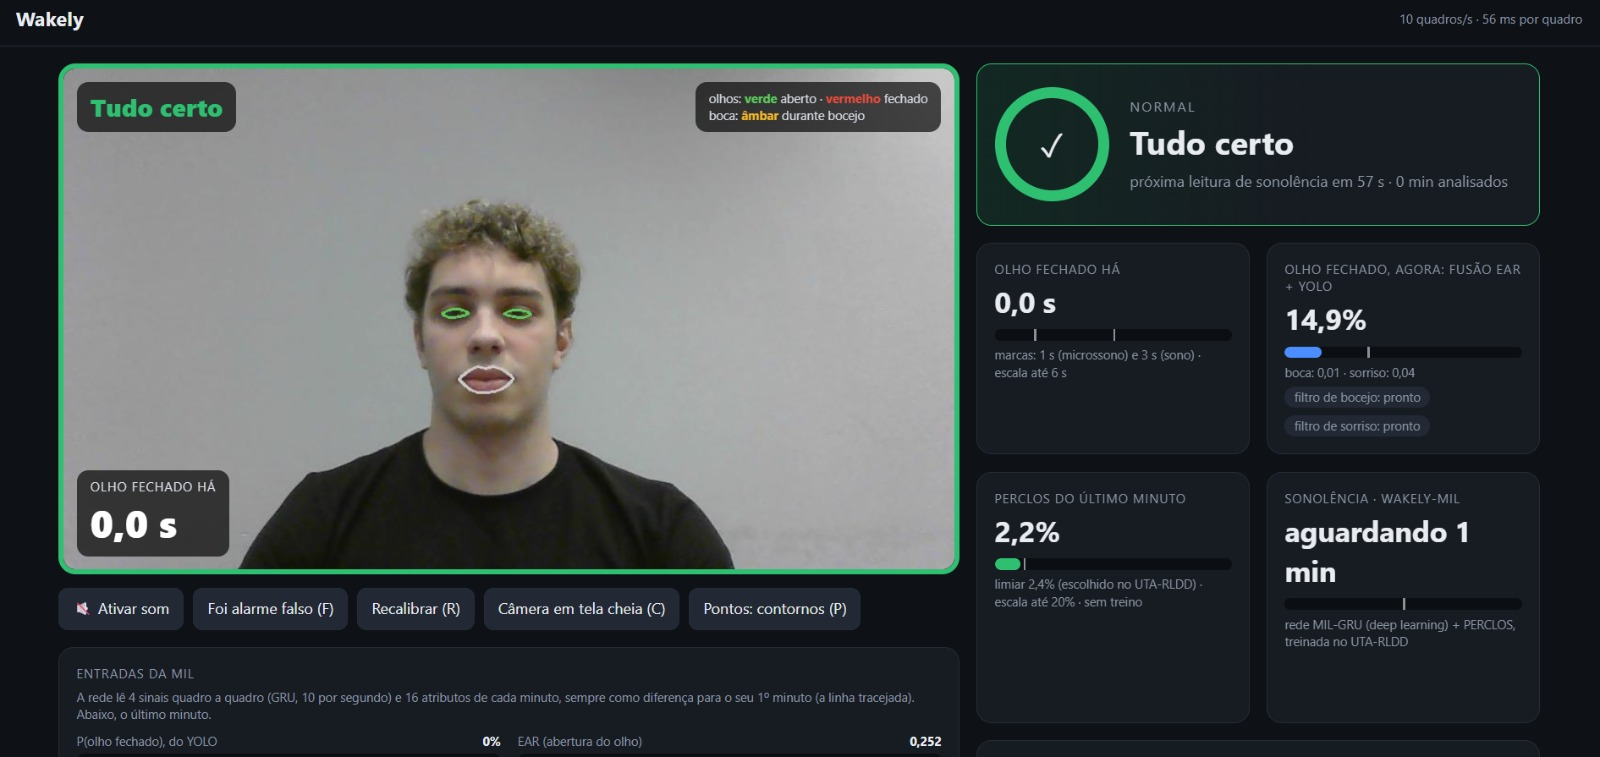
\includegraphics[width=\textwidth]{figs/painel_a.jpeg}\\[6pt]
\textbf{(b)}\\[2pt]
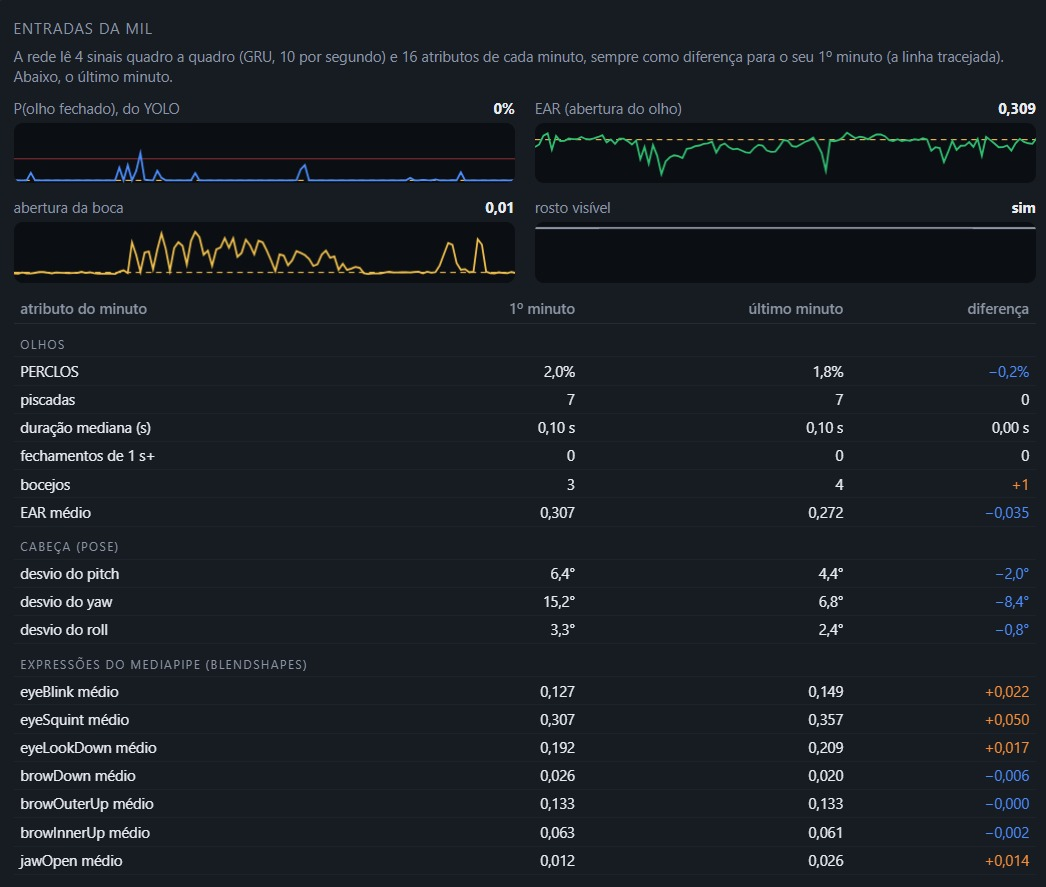
\includegraphics[width=0.7\textwidth]{figs/painel_b.jpeg}
\caption{\textbf{Painel da demo no navegador, em uso.} (a) Estado normal (``Tudo certo''): o vídeo espelhado com os olhos em verde (abertos) e a boca em contorno; à direita, o sinal de olho fechado da fusão EAR + YOLO (14,9\%, abaixo do limiar), o estado dos filtros de bocejo e de sorriso, o PERCLOS do último minuto (2,2\%, com o limiar de 2,4\% escolhido no UTA-RLDD) e o cartão do Wakely-MIL, que ainda aguarda 1 minuto de uso. (b) Cartão ``Entradas da MIL'': os quatro sinais por quadro do último minuto (P(fechado) do YOLO, EAR, abertura da boca e rosto visível) e, abaixo, os atributos do 1º minuto e do último minuto com a diferença, que é o que a rede lê. A pessoa na imagem é um integrante do grupo, que autorizou o uso.}
\label{fig:painel}
\end{figure}

Em testes, a regra ao vivo dá os mesmos alarmes da fusão offline nos 44 vídeos do FL3D e nos 8 do Eyeblink8. O pipeline roda a 12 a 19 quadros por segundo com a webcam de uma RTX 4060, e a webcam precisa de pelo menos 10 fps. Os tempos da máquina de estados (10 s sem rosto, 60 s de histerese, 5 min entre avisos de sonolência) são escolhas da demo e não foram validados. A demo não foi medida com motoristas.

%------------------------------------------------------------------
\section*{Ética e reprodutibilidade}
\label{sec:etica}

\paragraph{Ética.} O Wakely é um protótipo acadêmico, não um dispositivo de segurança, e nunca deve ser testado dirigindo. Gravações do grupo só em local seguro, na mesa ou em carro desligado e parado, e só como teste: treinar ou escolher limiar com elas faria o sistema decorar quem gravou. A calibração do primeiro minuto e a tecla de alarme falso são personalização na hora do uso. Vídeos da internet não foram usados, por violarem termos de uso e a LGPD. As bases têm restrições: o DROZY é só para pesquisa, sem redistribuir e sem mostrar imagens (citamos Massoz et al.~\cite{massoz2016}); a SUST-DDD não informa a licença dos vídeos; e a UL-DD tem acesso pessoal de um dos autores, com os dados só no disco dele, fora do Git. Por isso, \textbf{este trabalho não mostra nenhum quadro do DROZY, da SUST-DDD ou da UL-DD}. A licença do NITYMED diverge entre o Kaggle (CC BY-ND 4.0) e o DataPort (CC BY 4.0).

\paragraph{Reprodutibilidade.} O repositório é público, com licença AGPL-3.0, que atende à exigência da biblioteca Ultralytics. O comando é \texttt{uv sync} seguido de \texttt{uv run jupyter nbconvert --execute --inplace wakely.ipynb}. Com os caches prontos, a execução das seções 1 a 8 levava cerca de 17 minutos numa RTX 3050; sem cache, a primeira parte leva cerca de 1 hora (1,7 GB de download e 11 treinos), e a extração do UTA-RLDD leva cerca de 2,5 h na CPU de um Apple M5 (cerca de 2 h na extração rica, em um processo só). As seções 11 e 12 têm seus próprios caches e scripts em \texttt{experimentos/}. O notebook inteiro passa de 15,7 GB de memória e deve ser executado num terminal separado, ou em execução parcial. Os resultados dependem da máquina: o MediaPipe em Mac e em Windows e o arredondamento de CPU e GPU mudam um pouco os números (os falsos alarmes do YOLO com filtro foram de 10,2 para 9,4 no M5). Algumas checagens foram feitas fora do notebook (alinhamento com o NITYMED, inspeção visual dos recortes, extração da UL-DD), e o notebook registra só as conclusões. Os dados e os pesos não são versionados.

%------------------------------------------------------------------
\begin{thebibliography}{99}
\small
\setlength{\itemsep}{2pt}

\bibitem{soukupova2016} T.~Soukupová e J.~Čech. Real-time eye blink detection using facial landmarks. \emph{21st Computer Vision Winter Workshop}, 2016.

\bibitem{dinges1998} D.~F.~Dinges et al. Evaluation of techniques for ocular measurement as an index of fatigue and as the basis for alertness management. Relatório DOT HS 808 762, Departamento de Transportes dos EUA, 1998.

\bibitem{euroncap} Euro NCAP. \emph{Assessment Protocol: Safe Driving, Driver Engagement}, v1.2. \url{https://cdn.euroncap.com/cars/assets/Euro_NCAP_Protocol_Safe_Driving_Driver_Engagement_v1_2_ebce03a443.pdf}

\bibitem{skorucak2020} J.~Skorucak et al. Automatically detected microsleep episodes in the fitness-to-drive assessment. \emph{Frontiers in Neuroscience}, 14:8, 2020. doi:10.3389/fnins.2020.00008.

\bibitem{boyle2008} L.~N.~Boyle et al. Driver performance in the moments surrounding a microsleep. \emph{Transportation Research Part F}, 2008.

\bibitem{ghoddoosian2019} R.~Ghoddoosian, M.~Galib e V.~Athitsos. A realistic dataset and baseline temporal model for early drowsiness detection. \emph{CVPR Workshops}, 2019. arXiv:1904.07312.

\bibitem{massoz2016} Q.~Massoz, T.~Langohr, C.~François e J.~G.~Verly. The ULg multimodality drowsiness database (called DROZY) and examples of use. \emph{IEEE WACV}, 2016.

\bibitem{massoz2018} Q.~Massoz, J.~G.~Verly e M.~Van Droogenbroeck. Multi-timescale drowsiness characterization based on a video of a driver's face. \emph{Sensors}, 18(9), 2018.

\bibitem{revisao126} E.~Perkins, C.~Sitaula, M.~Burke e F.~Marzbanrad. Challenges of driver drowsiness prediction: the remaining steps to implementation. arXiv:2109.08355, 2021.

\bibitem{anund2013} A.~Anund, C.~Fors, D.~Hallvig, T.~Åkerstedt e G.~Kecklund. Observer rated sleepiness and real road driving: an explorative study. \emph{PLoS ONE}, 8(5):e64782, 2013. doi:10.1371/journal.pone.0064782.

\bibitem{ilse2018} M.~Ilse, J.~M.~Tomczak e M.~Welling. Attention-based deep multiple instance learning. \emph{ICML}, 2018.

\bibitem{fl3d} Frame Level Driver Drowsiness Detection (FL3D). Conjunto de dados no Kaggle, derivado do NITYMED (autoria não informada na página). \url{https://www.kaggle.com/datasets/matjazmuc/frame-level-driver-drowsiness-detection-fl3d}

\bibitem{nitymed} N.~Petrellis et al. NITYMED: night-time yawning-microsleep-eyeblink-driver distraction dataset. IEEE DataPort. doi:10.21227/85xe-3f88.

\bibitem{eyeblink8} T.~Drutarovský e A.~Fogelton. Eye blink detection using variance of motion vectors. \emph{ECCV Workshops}, pp.~436--448, 2014. (Introduz o Eyeblink8.)

\bibitem{sustddd} E.~Kavalci Yilmaz e M.~A.~Akcayol. SUST-DDD: a real-drive dataset for driver drowsiness detection. \emph{31st Conference of Open Innovations Association (FRUCT)}, pp.~416--421, 2022. doi:10.5281/zenodo.6519933.

\bibitem{uldd} M.~Bodaghi, M.~Hosseini, R.~Gottumukkala, R.~T.~Bhupatiraju, I.~Ahmad e M.~Gabbouj. UL-DD: a multimodal drowsiness dataset using video, biometric signals, and behavioral data. arXiv:2507.13403, 2025.

\bibitem{mediapipe} C.~Lugaresi et al. MediaPipe: a framework for building perception pipelines. arXiv:1906.08172, 2019.

\bibitem{howard2019} A.~Howard et al. Searching for MobileNetV3. \emph{ICCV}, 2019.

\bibitem{ultralytics} Ultralytics. YOLO26. \url{https://docs.ultralytics.com/models/yolo26/}

\end{thebibliography}

\end{document}
